\chapter{FireCube数据集及变量分析}
\label{chap:dataset}
有一些公开的数据集可以用于野火风险预测，但它们在解决的任务、观测变量、空间和时间分辨率上存在显著差异。本文选择FireCube数据集作为使用的数据集，它由 Prapas 发布\cite{prapas2021deep}、Kondylatos 扩展与改进\cite{kondylatos2022wildfire}，并最终由\textcite{prapas2022firecube}分类整理为 2D 和 3D 格式，可在zenodo网站\cite{prapas2022firecube_dataset}得到。观测变量包括气象数据、卫星衍生数据、地形特征、人类相关活动以及历史火灾记录。此外，还提供了土地覆盖类型（CLC）和火险指数（FWI）。任务目标是预测每个像素的野火是否会在第二天燃起并扩大规模，该任务相当于对每一个像素点的二元分类任务，判断该像素点是否发生野火事件。

\section{区域概况及时空数据构建}
\label{sec:regional-overview-and-spatio-temporal-data-construction}
FireCube数据集定义了一个像素级别的野火预测任务，包含了从2009年至2021年间90个变量的多变量时空数据流，分辨率为$1km\times 1km\times 1day$。我们选择FireCube数据集，其以希腊作为研究地点。因为希腊展现出独特的野火模式和环境特征，使其成为野火预测和驱动因素的理想案例研究。希腊位于地中海气候区，夏季炎热干燥，极易发生野火。此外，其复杂的地形、植被分布以及人类活动的影响进一步加剧了野火风险和破坏性。数据集所定义的区域面积为$1253km\times 983km$，包括希腊及东地中海部分地区。

野火数据来源于 EFFIS 的历史过火面积数据\cite{san2013european}以及 MODIS 的活跃火点产品\cite{giglio2016collection}。该数据集对这两类数据进行了空间交叉（spatial intersection）分析，以重建火灾的起火日期。通过将活跃火点与过火面积相互关联，确定了每场野火的起火日期，并将属于同一野火事件的燃烧面积进行合并。为了确定起火日期，研究会在燃烧面积的矢量数据周围创建一个 1 公里的缓冲区，并在此缓冲区内，搜索在 EFFIS 记录的起火日期前一周内所生成的活跃火点。

\section{采样方式及训练数据}
\label{sec:sampling-method-and-training-data}
由于野火风险预测本质上是一项不平衡分类任务，其中正样本的数量远少于负样本，因此为了便于模型训练，需要对原始数据进行采样，构建训练样本，并划分训练集，验证集，测试集。研究\cite{kondylatos2022wildfire}的作者按照如下方式提取样本：对于目标日$T+1$，对于目标像素$1km\times 1km$的格点，静态变量形成一个以目标像素为中心的$25km\times 25km$的斑块；动态变量由从$T-9$天到$T$的$25km\times 25km\times 10day$时间序列组成。每个样本均包含数个静态变量与动态变量，因此本任务本质上属于前文第\ref{sec:1-2-spatiotemporal-prediction}节中所述的时空预测问题。其中正样本代表该目标像素点发生野火事件，负样本代表该目标像素点未发生野火事件。对于每个正样本，会从不同地点抽取少量负样本，负样本有两种来源，一是随机抽取，二是从与正样本土地覆盖类型相似的地区抽样，以提高任务难度。

图\ref{fig:2-2-samples}展示了数据集中各年份正负样本的数量分布。总体而言，2009年至2020年间的样本总量保持相对均衡，然而，2021年的数据量出现了显著的激增。这一异常增长主要归因于2021年夏季在希腊地区爆发的规模空前、破坏力极强的极端野火事件\cite{giannaros2022meteorological}。总体数据包括71471个训练样本，其中包含13518个正样本和57953个负样本，来自2009年-2018年的原始数据；6430个验证样本，其中包含1300个正样本和5130个负样本，均来自2019年；42820个测试样本，其中包含2020年的1228个正样本、4860个负样本和2021年4407个正样本、32325个负样本。训练样本、验证样本和测试样本构成模型训练评估时的训练集，验证集，测试集。提取的训练数据可在\cite{prapas2022training}中获取。在深度学习理论中，训练集是用于模型内部参数（Parameters）估计或学习的数据样本集合，验证集是用于模型选择和超参数调优（Hyperparameter Tuning）的数据样本集合，测试集是用于对最终选定的最优模型进行泛化误差估计的数据样本集合\cite{bengio2017deep}。
\begin{figure}[htbp]
    \centering
    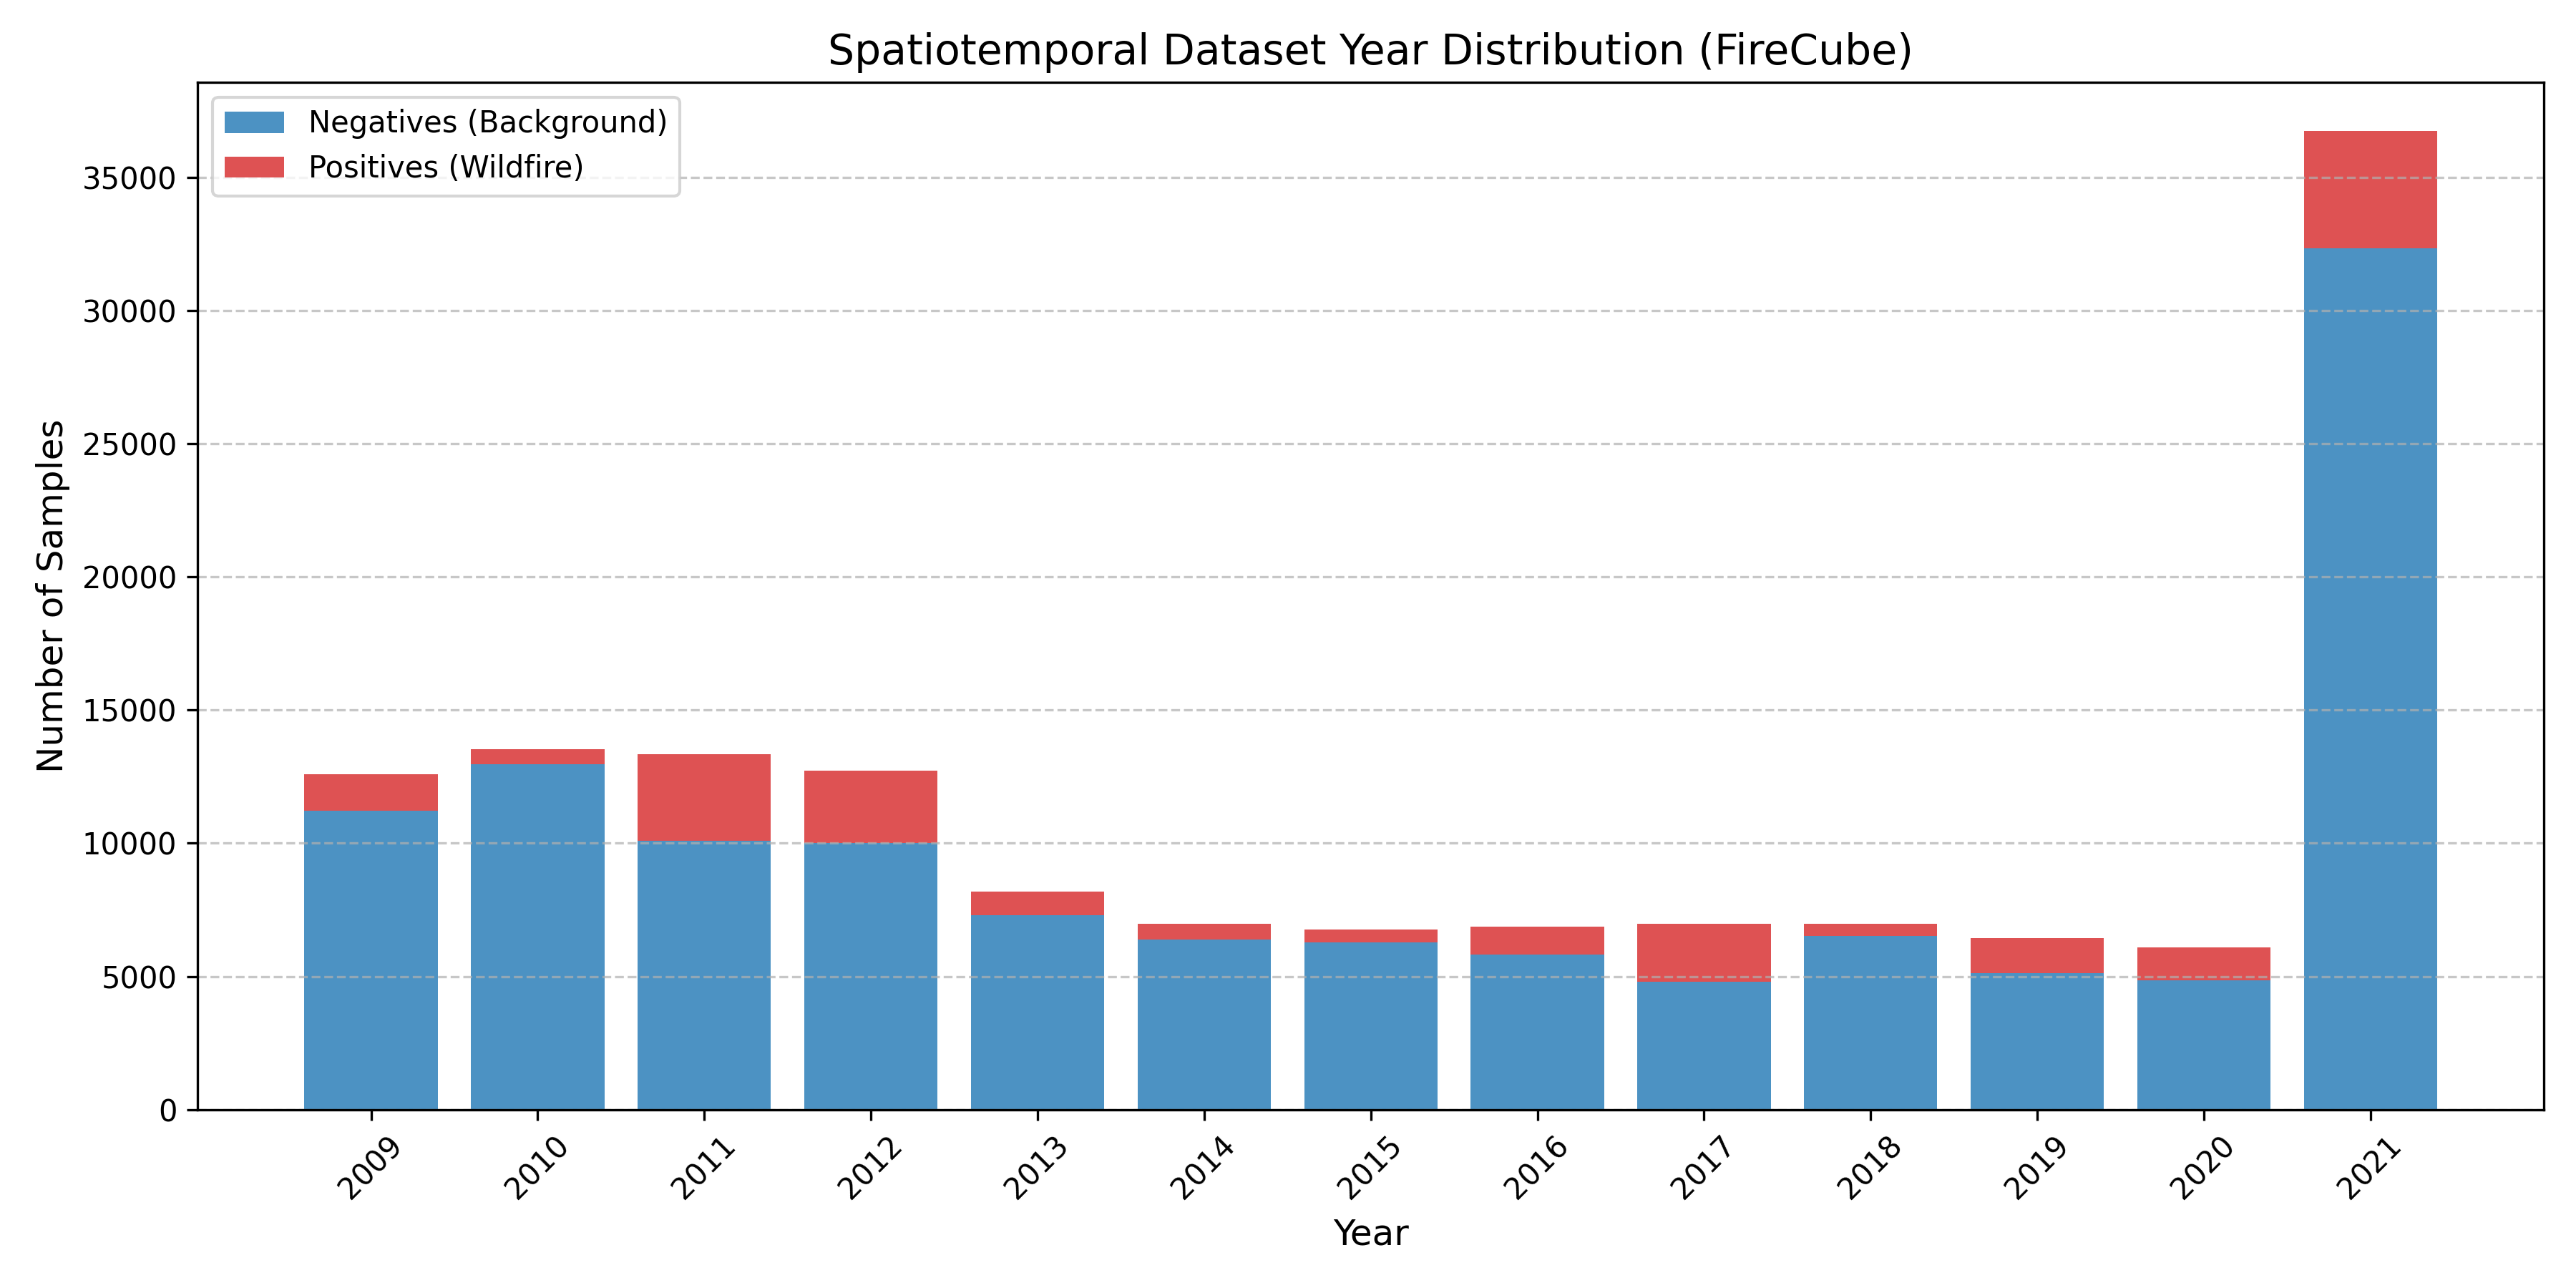
\includegraphics[width=0.9\textwidth]{img/chap2/2-2-samples.png}
    \caption{FireCube训练数据中各年份采样的样本数量}
    \label{fig:2-2-samples}
\end{figure}

同时，原始数据集虽然包含了90个变量，但其中存在大量的时间切片冗余，如不同年份的的静态背景数据以及统计维度的相似性（如同一气象指标的最高、最低和平均值），为了降低模型复杂度，避免维度灾难以及共线性带来的过拟合问题，FireCube数据集对原始变量进行整合和缩减，最终保留了25个变量，其中包含15个静态变量和10个动态变量。表\ref{tab:static_vars}展示了数据集静态特征变量列表，分别包含地形特征、水文与人类活动和地表覆盖变量三个大类，其中地表覆盖变量采用one-hot独热编码，详细的地表覆盖类型及物理含义如表\ref{tab:clc_vars}所示。

\begin{table}[htbp]
    \centering
    \caption{FireCube 数据集静态特征变量列表}
    \label{tab:static_vars}
    \renewcommand{\arraystretch}{1.5} 
    \begin{tabularx}{\textwidth}{
        >{\raggedright\arraybackslash}p{2.8cm} 
        >{\raggedright\arraybackslash}p{4.5cm} 
        >{\raggedright\arraybackslash}p{2.5cm} 
        >{\raggedright\arraybackslash}X }
        \toprule
        \textbf{变量大类} & \textbf{变量名称} & \textbf{中文名称} & \textbf{物理含义} \\
        \midrule
        
        \textbf{地形特征} 
        & Digital elevation model (DEM) & 数字高程模型 & 表征海拔高度，影响局地气候与植被的垂直分布 \\
        & Slope & 坡度 & 影响野火蔓延的动力学特征 \\
        \midrule
        
        \textbf{水文与人类活动} 
        & Distance to waterway & 与水域的距离 & 反映地表可用水源分布及天然防火隔离带的邻近程度 \\
        & Distance to roads & 与道路的距离 & 衡量人类活动的可达性与基础设施分布 \\
        & Population density & 人口密度 & 表征区域人口聚集度，反映人类活动对自然环境的干扰强度 \\
        \midrule
        
        \textbf{地表覆盖变量}
        & 10 Copernicus Corine Land Cover variables & 10 类地表覆盖类型 & 表征地表可燃物类型与空间分布基底（包含森林、灌木、人造表面等10个具体子类，详见表 \ref{tab:clc_vars}） \\
        
        \bottomrule
    \end{tabularx}
\end{table}


\begin{table}[htbp]
    \centering
    \caption{FireCube 数据集地表覆盖变量 (CLC) 详细分类}
    \label{tab:clc_vars}
    \renewcommand{\arraystretch}{1.5} 
    % CLC 表格同样采用顶部对齐
    \begin{tabularx}{\textwidth}{ 
        >{\raggedright\arraybackslash}p{4.2cm} 
        >{\raggedright\arraybackslash}p{3cm} 
        >{\raggedright\arraybackslash}X }
        \toprule
        \textbf{变量名称} & \textbf{中文名称} & \textbf{物理含义} \\
        \midrule
        
        Artificial ground & 人造表面 & 连续的城市结构、工业或商业单元、公路和铁路网络及相关土地、港口区域、机场、矿产开采场、垃圾场、建筑工地、城市绿地、体育和休闲设施 \\
        \midrule
        
        Discontinuous urban fabric & 城市不连续表面 & 不连续的城市，如城镇边缘、绿化带等 \\
        \midrule
        
        Arable land & 可耕种地 & 非灌溉耕地、永久灌溉土地、稻田 \\
        \midrule
        
        Permanent crops & 永久耕地 & 果园、葡萄园等农业用地 \\
        \midrule
        
        Pastures & 牧场 & 牧场、天然或人工草地 \\
        \midrule
        
        General agriculture & 普通农用地 & 与永久作物相关的一年生作物、复杂种植模式的作物、大面积自然植被覆盖的主要用于农业的土地 \\
        \midrule
        
        Forests & 森林 & 阔叶林、针叶林、混交林 \\
        \midrule
        
        Miscellaneous vegetation & 植被杂项 & 自然草地、荒原、硬叶植被、过渡林和灌木 \\
        \midrule
        
        Miscellaneous without vegetation & 无植被杂项 & 沙地、裸岩、极稀疏植被、烧毁区域、冰川、全年积雪区域 \\
        \midrule
        
        Water & 水体 & 内陆沼泽、泥炭沼泽、盐沼、潮间带泥滩、沿海泻湖、河口、海洋和湖泊 \\
        \bottomrule
    \end{tabularx}
\end{table}

表\ref{tab:dynamic_vars}展示了FireCube 数据集动态特征变量列表，包含气温与热力、湿度与降水、空气动力与气压、植被与土壤四个大类的特征变量。值得一提的是，虽然\textcite{prapas2022training}构造的训练数据包含25个特征变量，但其余变量依然在数据集中，只是没有被选择输入到深度学习神经网络中，例如原始数据中包含最大经向风速（$max\_wind\_v10$）和最大纬向风速（$max\_wind\_u10$），而作者选择保留了最大风速（$max\_wind\_speed$）作为输入。但是，我们可以从经向风速和纬向风速中提取出风向的信息，从而对野火蔓延预测提供指导，因此，在后续进行改进与分析时可能会使用更多特征变量。

\begin{table}[htbp]
    \centering
    \caption{FireCube 数据集动态特征变量列表}
    \label{tab:dynamic_vars}
    % 拉大行高，保持呼吸感
    \renewcommand{\arraystretch}{1.5} 
    % 全部改用 p 列（顶部对齐），加入 \raggedright 防止文字被强行拉伸溢出
    \begin{tabularx}{\textwidth}{
        >{\raggedright\arraybackslash}p{2.8cm} 
        >{\raggedright\arraybackslash}p{4.5cm} 
        >{\raggedright\arraybackslash}p{2.5cm} 
        >{\raggedright\arraybackslash}X }
        \toprule
        \textbf{变量大类} & \textbf{变量名称} & \textbf{中文名称} & \textbf{物理含义} \\
        \midrule
        
        \textbf{气温与热力} 
        & Maximum 2m temperature & 2m最高温度 & 表征大气最热时段的热力学状态 \\
        & Day land surface temperature & 日间地表温度 & 卫星反演的白天陆地表面温度 \\
        & Night land surface temperature & 夜间地表温度 & 卫星反演的夜间陆地表面温度 \\
        \midrule
        
        \textbf{湿度与降水} 
        & Maximum 2 m dew point temperature & 2m最高露点温度 & 反映近地表空气中的绝对水汽含量 \\
        & Minimum relative humidity & 最小相对湿度 & 表征空气的极端干燥程度\\
        & Total precipitation & 日总降水量 & 反映地表水分补充情况\\
        \midrule
        
        \textbf{空气动力与气压} 
        & Maximum wind speed & 最大风速 & 影响野火推进速率与方向 \\
        & Maximum surface pressure & 最高表面气压 & 反映大尺度天气系统的状态 \\
        \midrule
        
        \textbf{植被与土壤} 
        & Normalized difference vegetation index (NDVI) & 归一化植被指数 & 反映植被覆盖度与生长活力，表征地表可燃物的现存状态 \\
        & Soil moisture index (sminx) & 土壤湿度指数 & 衡量地表及浅层土壤的干旱缺水程度 \\
        
        \bottomrule
    \end{tabularx}
\end{table}

\section{特征变量分析}
\label{sec:characteristic-variable-analysis}
本节通过探索性数据分析（Exploratory Data Analysis，EDA）揭示野火发生与环境因子之间的内在联系，为模型的设计提供依据。
\subsection{静态变量分析}
\label{sec:static-variables-analysis}
图\ref{fig:2-3-monthly-distribution}展示了研究区域内野火发生频次的月度分布情况。从图中可以清晰地观察到，野火的发生呈现出极强的季节性聚集特征。全年绝大多数的火灾集中爆发在夏季和初秋，其中 8月份 是火灾风险的绝对高峰期，单月发生频次占到了总样本的 56.0\%，紧随其后的是 7月（22.8\%）和 9月（11.1\%）。这三个月累计贡献了全年近 90\% 的火灾事件。相反，在 11月至次年 5月的冬春季节，火灾发生率极低，各月占比均不足 1\%。

\begin{figure}[H]
    \centering
    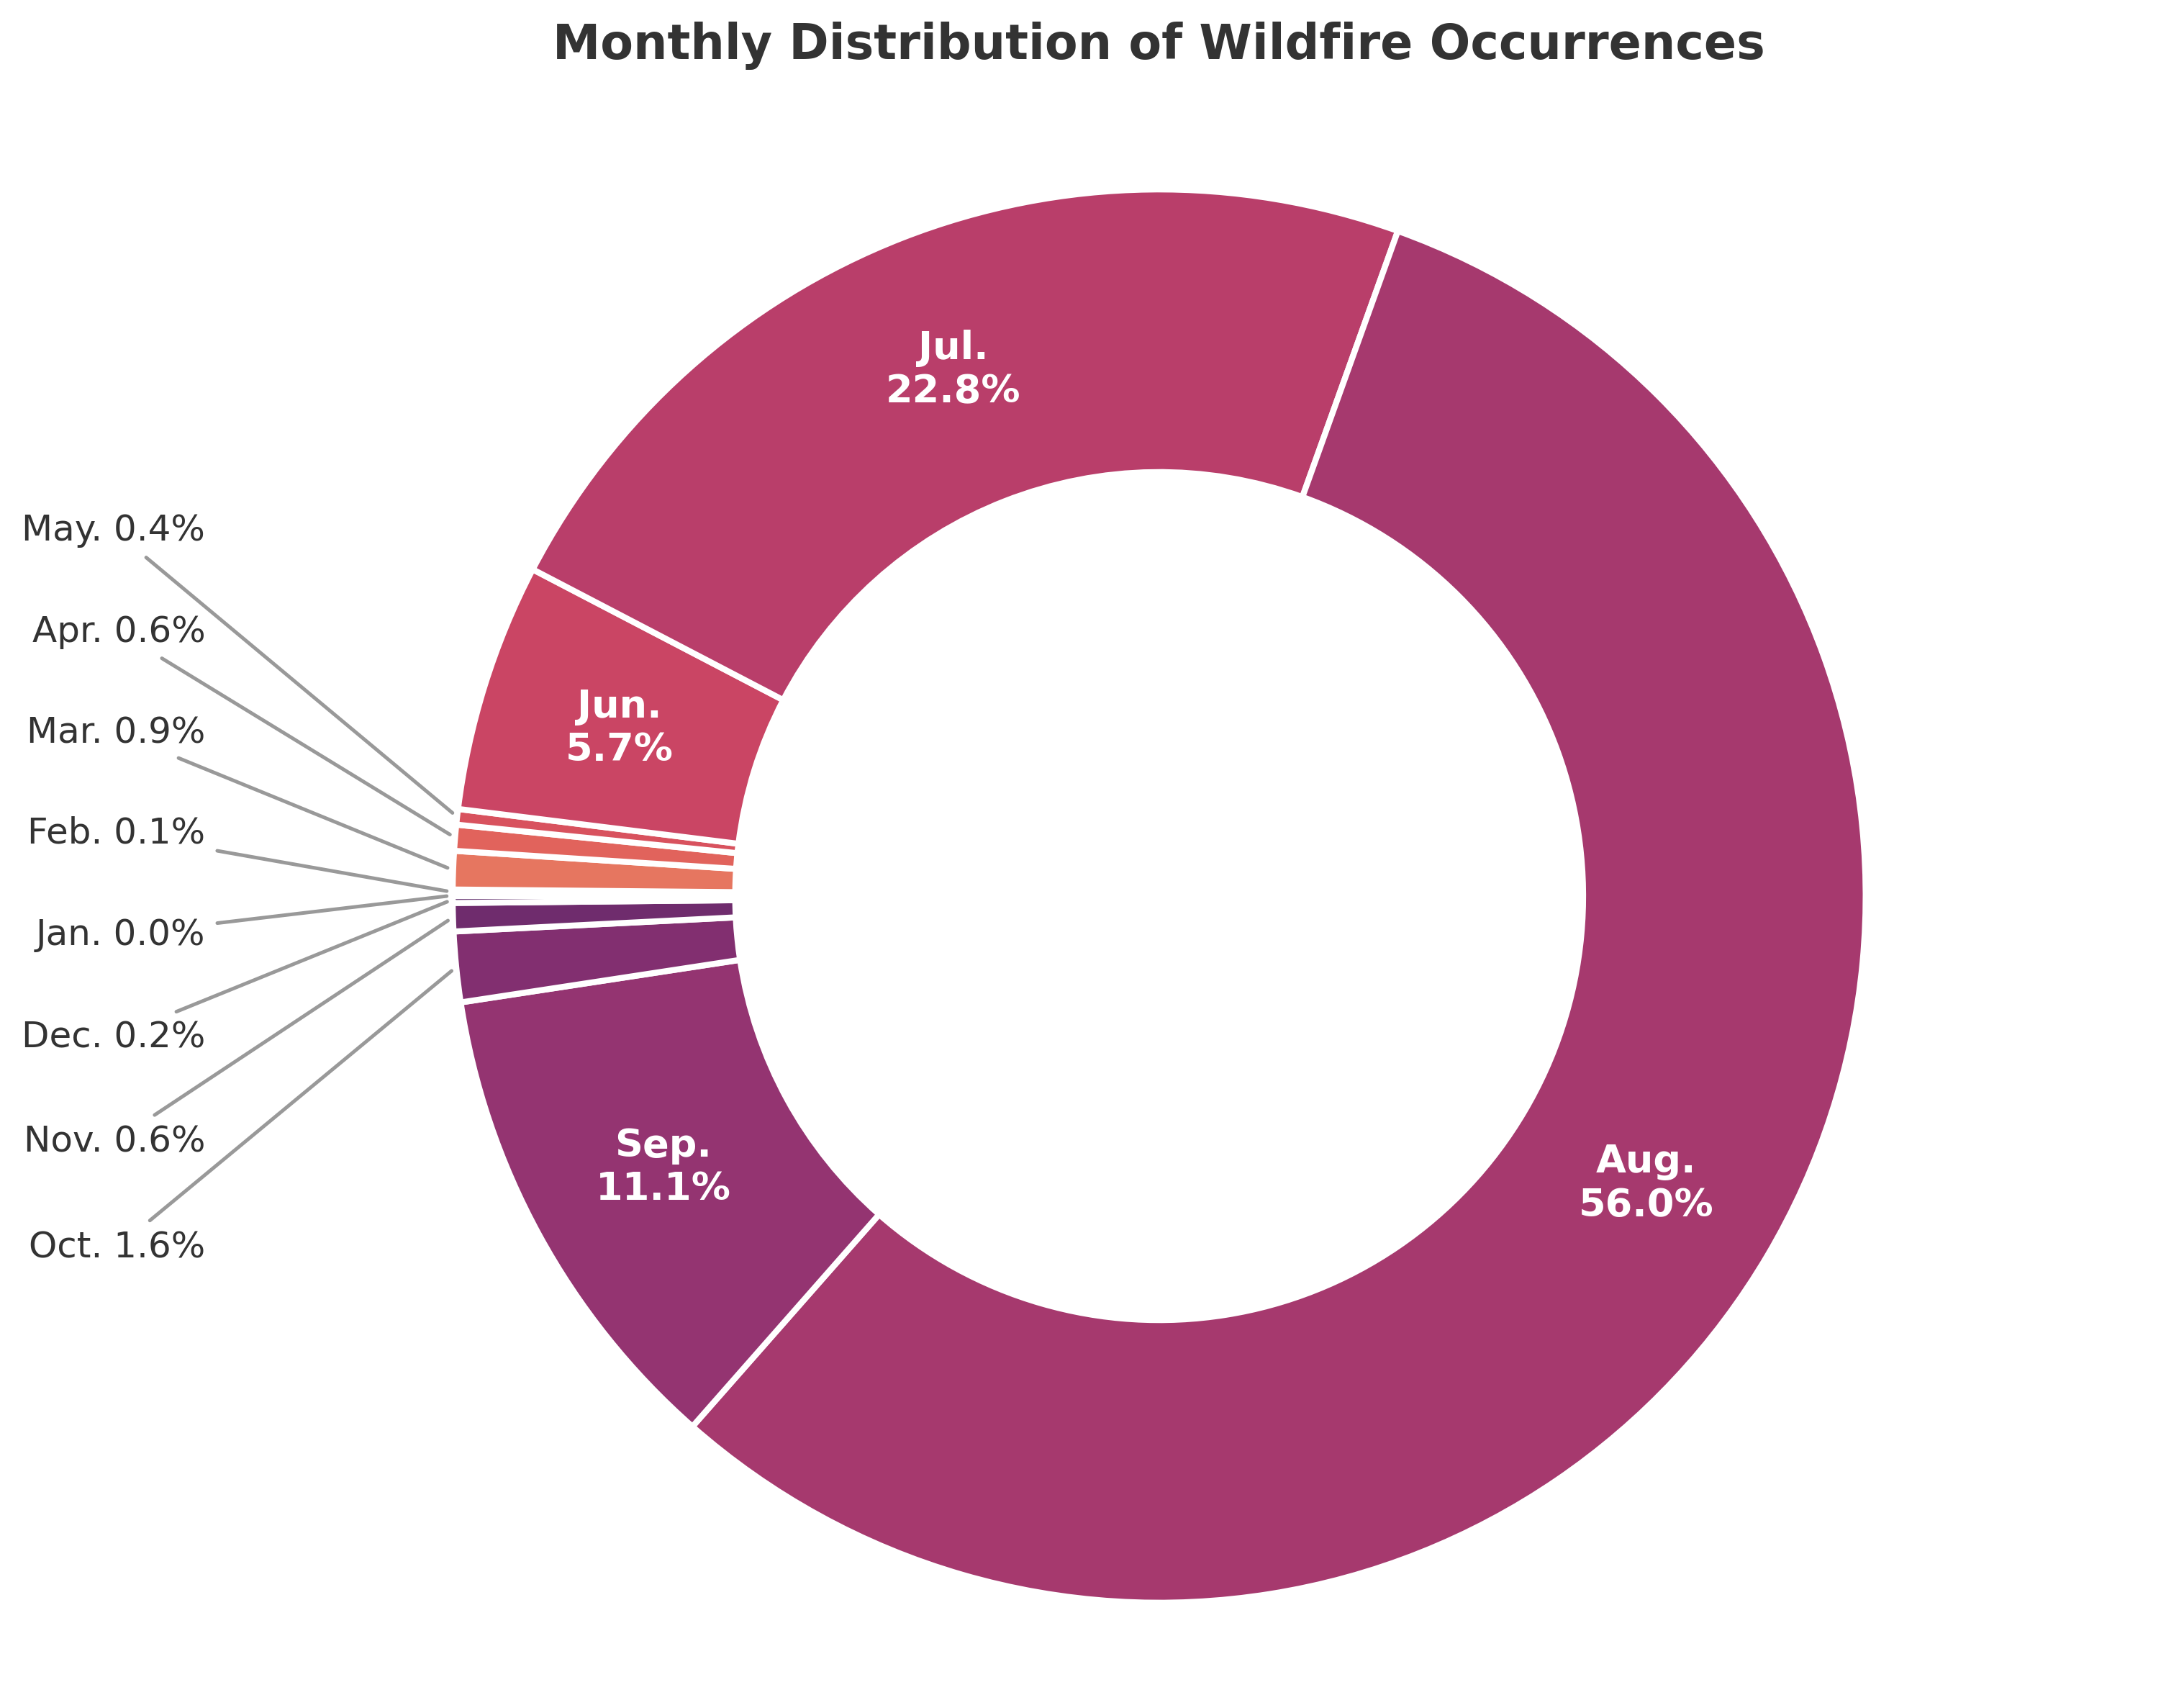
\includegraphics[width=0.9\textwidth]{img/chap2/2-3-monthly-distribution.png}
    \caption{FireCube数据集中野火发生频次的月度分布}
    \label{fig:2-3-monthly-distribution}
\end{figure}

这种极端的分布规律与该地区典型的地中海气候高度吻合。盛夏时期受副热带高压控制，持续的高温与稀少的降水导致地表植被含水量急剧下降，形成了极其易燃的环境，而冬春季节受西风带影响，降水充沛，环境湿度大，有效抑制了火灾的发生。

图\ref{fig:2-3-clc}展示了野火在不同 Corine 土地覆盖 （CLC）类型上的空间分布规律。从统计结果可以清晰地看到，野火的发生地点具有极强的植被选择性。其中，植被杂项（Miscellaneous vegetation）是火灾最密集的区域，其正样本数量以绝对优势位居第一，说明火灾易发生在混合植被与灌木草地，也说明该区域此种土地覆盖类型可能较多；其次是森林（Forests）与普通农用地（General agriculture）。相对而言，城市不连续表面（Discontinuous urban fabric）、人造表面（Artificial ground）以及无植被杂项（Miscellaneous without vegetation）发生火灾的频次极低。

\begin{figure}[htbp]
    \centering
    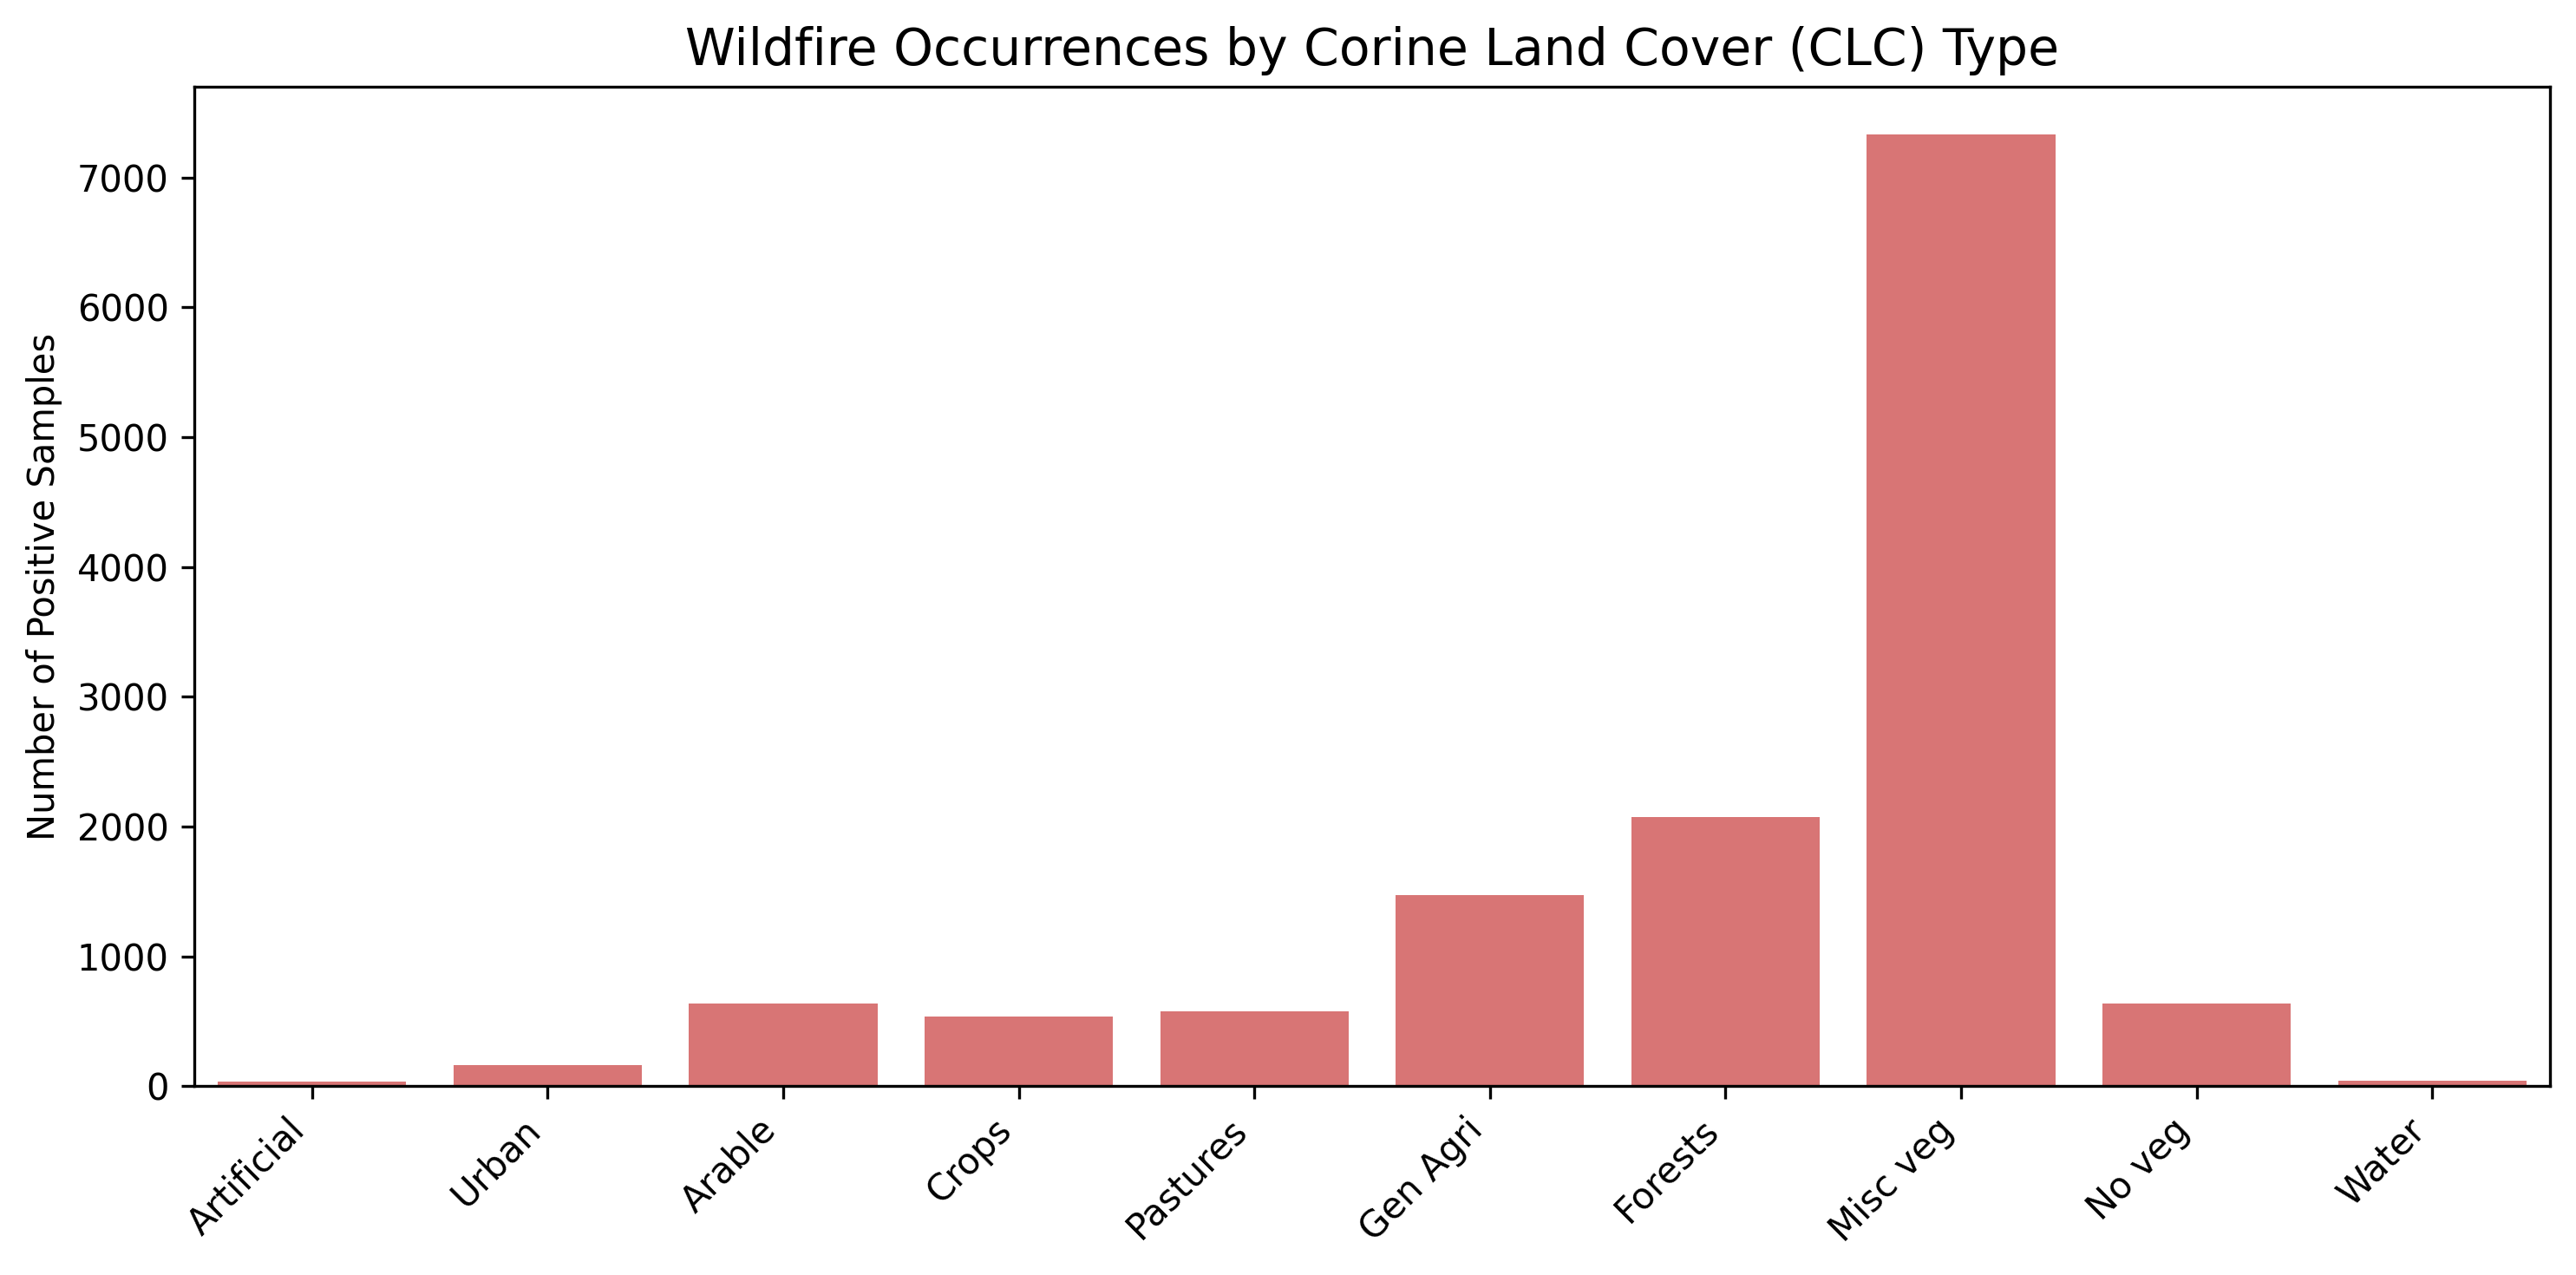
\includegraphics[width=0.9\textwidth]{img/chap2/2-3-clc.png}
    \caption{FireCube数据集中野火事件在不同土地覆盖类型(CLC)上的空间分布}
    \label{fig:2-3-clc}
\end{figure}

这一分布特征为本研究的模型架构设计提供了物理支撑。分布证明了地表覆盖类型，本质上是燃料基底的差异，对野火的发生具有较大的约束作用。这就要求模型必须具备独立剥离并感知这种地理底色的机制，而这恰恰是我们在架构中单独采用静态编码器分支，进行地貌特征提取的核心动机。

图\ref{fig:2-3-elevation-slope}展示了研究区域内野火发生频次在海拔（Elevation）与坡度（Slope）两个静态地理维度上的二维核密度分布。

\begin{figure}[htbp]
    \centering
    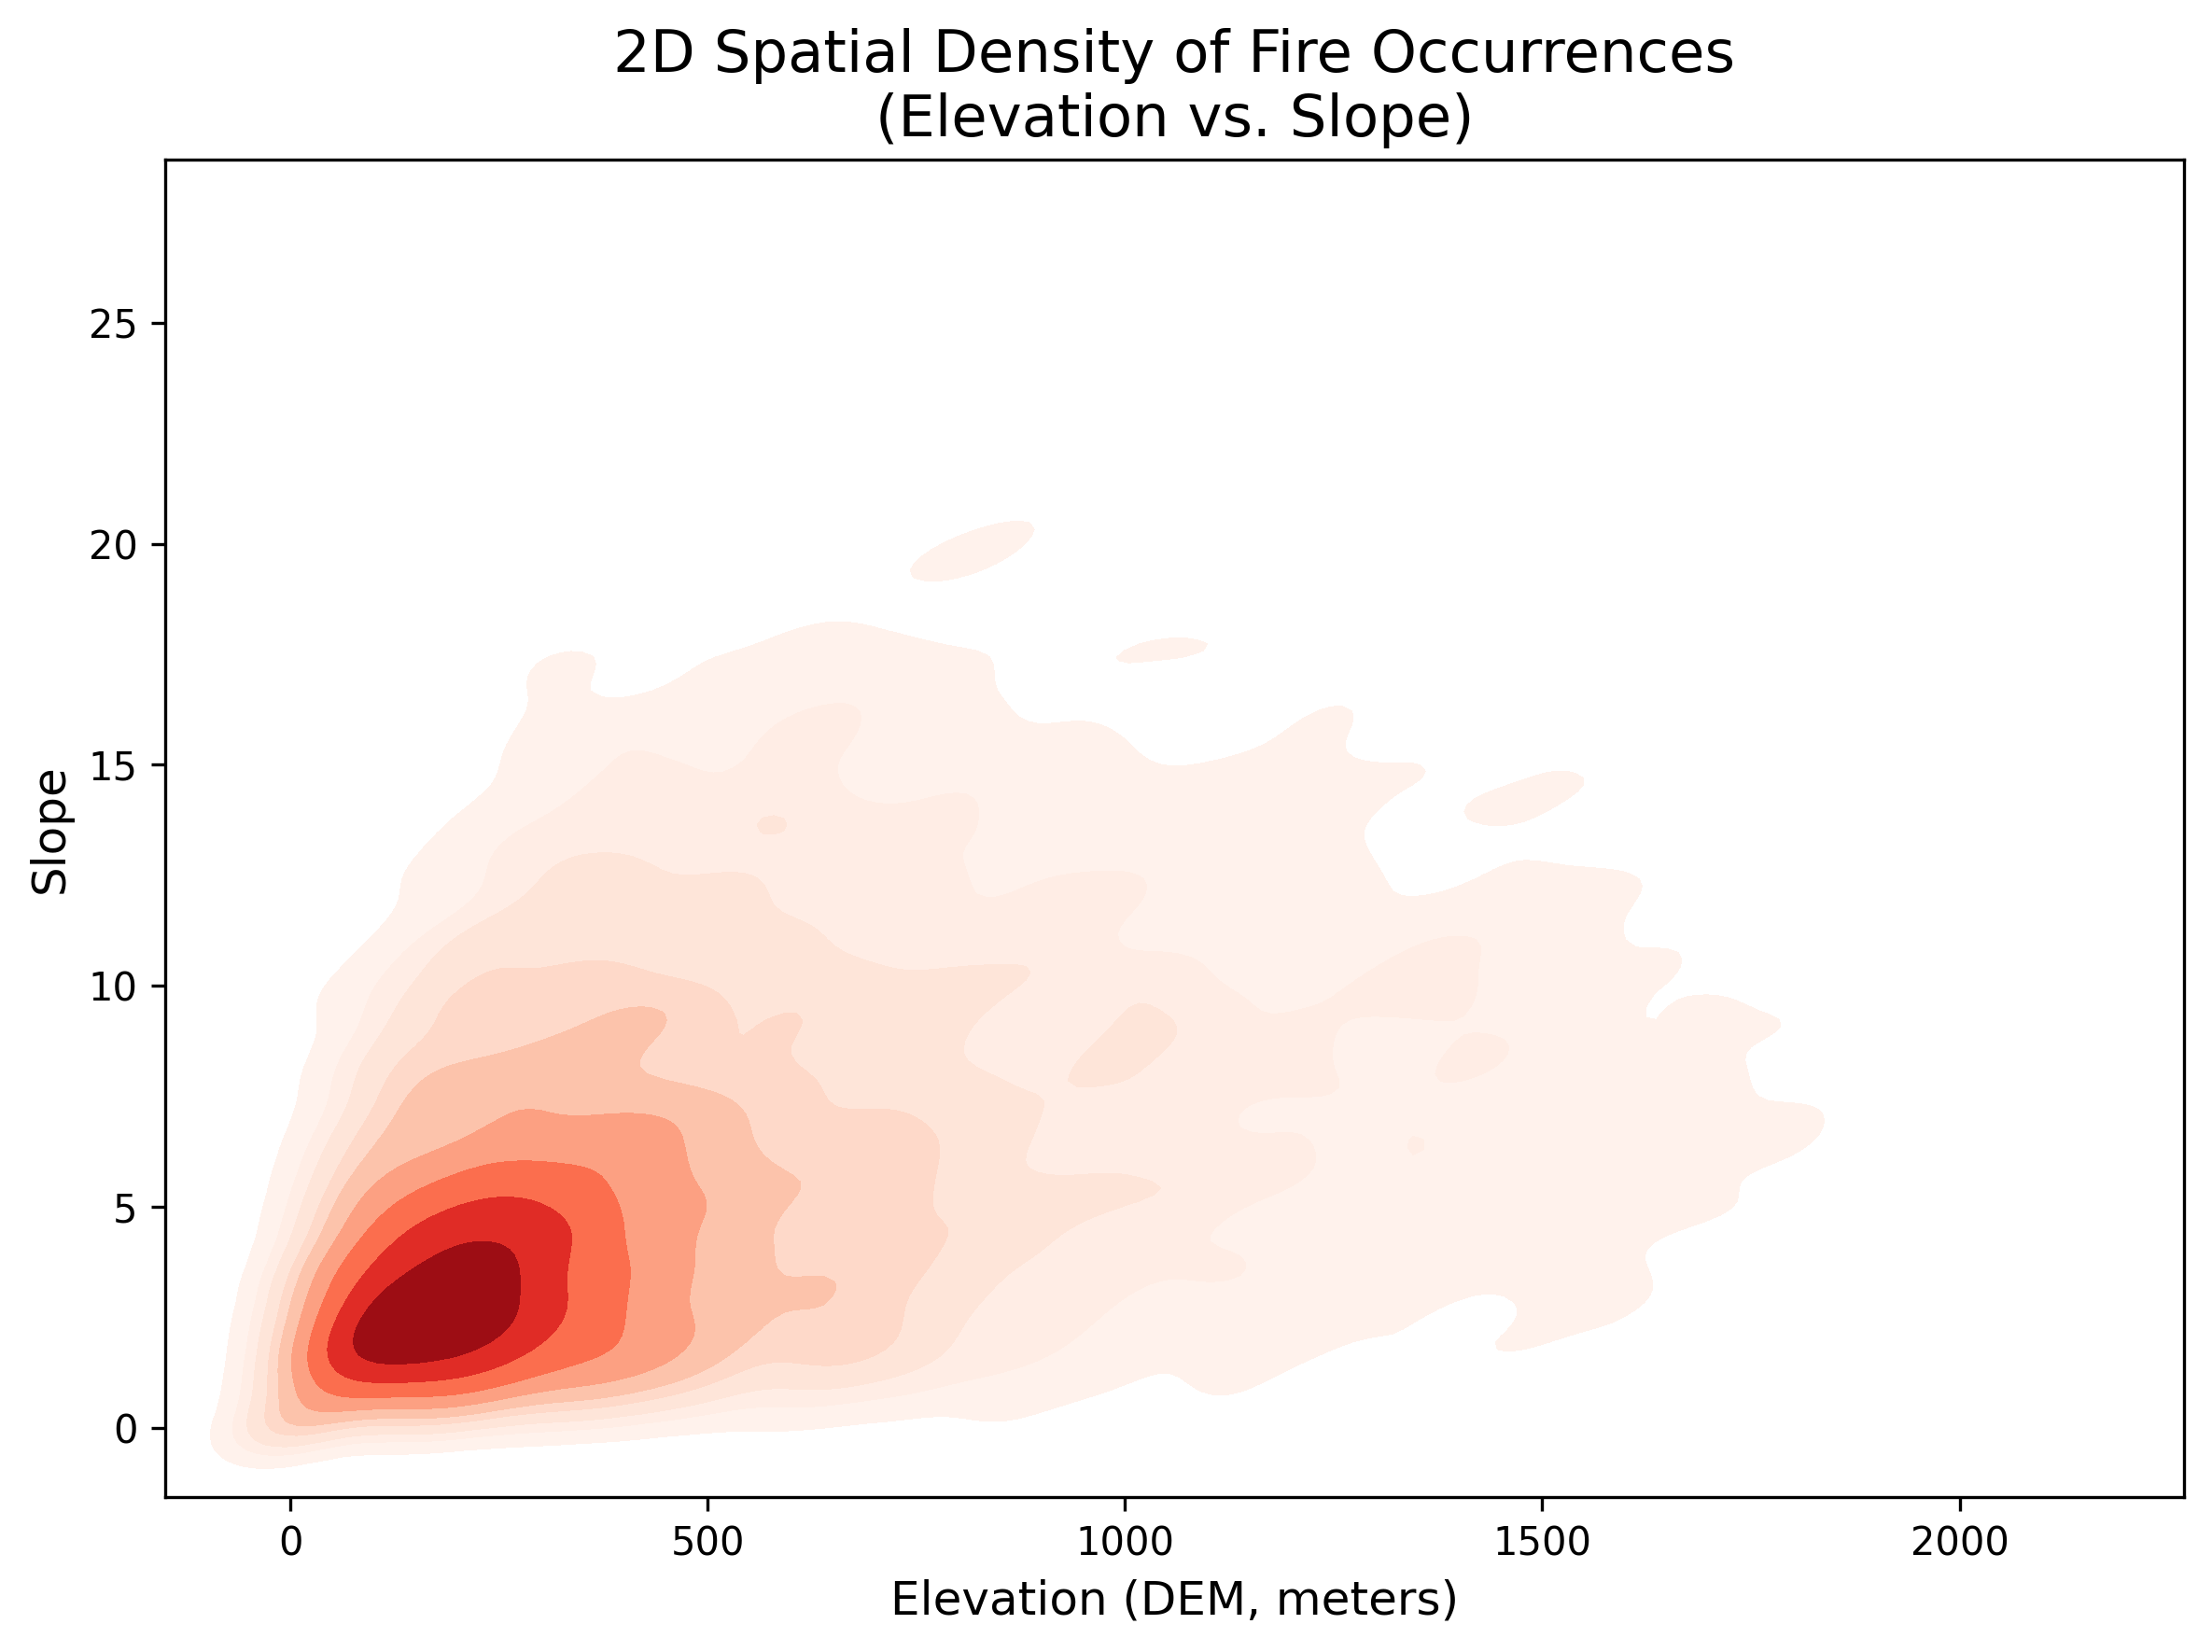
\includegraphics[width=0.8\textwidth]{img/chap2/2-3-elevation-slope.png}
    \caption{FireCube数据集中野火海拔与坡度上的二维核密度分布}
    \label{fig:2-3-elevation-slope}
\end{figure}
从图中的密度分布可以清晰地观察到，野火主要发生在海拔较低（约 0-400 米）且坡度平缓（约 0-5 度）的区域。随着海拔的升高或坡度的增加，颜色迅速变浅，说明一旦海拔升高或在陡坡地区，火灾发生频次就会断崖式下降。造成这一地理分布特征可能是因为，低海拔地区在火灾季通常有更高的气温和更强的蒸发作用，形成了易燃的环境，并且低海拔与平缓坡地往往是人类定居点、农业用地和路网密集的区域，人类活动增加了火源出现的概率。

\subsection{动态变量分析}
\label{sec:dynamic-variable-analysis}
图\ref{fig:2-3-correlation-matrix}展示了FireCube数据集正样本中的10类动态特征变量的皮尔逊相关性矩阵热力图。通过对相关性系数的分析，可以揭示气象因子在火灾发生时可能的物理机制。

首先，热力图展现了火险天气的典型特征。其中，最高气温（$Max\_t2m$）与最低相对湿度（$Min\_rh$）呈现出全图最强的负相关性（$r=−0.50$）。这符合火灾发生前的物理规律：气温的异常升高往往伴随着空气水分的剧烈蒸发，导致相对湿度骤降，从而极大地加速了地表可燃物的干燥过程。此外，最大地表气压（$Max\_sp$）与最大风速（$Max\_wind$）呈现出显著的正相关（$r=0.57$），表明气压梯度的变化是驱动大风、进而助长火势蔓延的重要动力学因素。其次，土壤湿度（$sminx$）表现出了较强的特征独立性，这表明土壤湿度是一个刻画长期干旱累积效应的变量，其变化较慢，它提供了区别于快速气象变化的独特物理信息。最后，从深度学习特征工程的角度来看，该图证明了选取的特征集合的优质性。矩阵中所有非对角线元素的绝对值均未超过0.6，表明这些动态特征之间不存在严重的多重共线性（Multicollinearity）。这说明本文选取的 10 个动态特征各自包含了相对独立的信息，特征冗余度低。这一发现确保了后续输入Swin Transformer网络的数据质量，有助于模型更稳定、高效地提取时空演变特征。

\begin{figure}[htbp]
    \centering
    \begin{minipage}{0.48\textwidth}
        \centering
        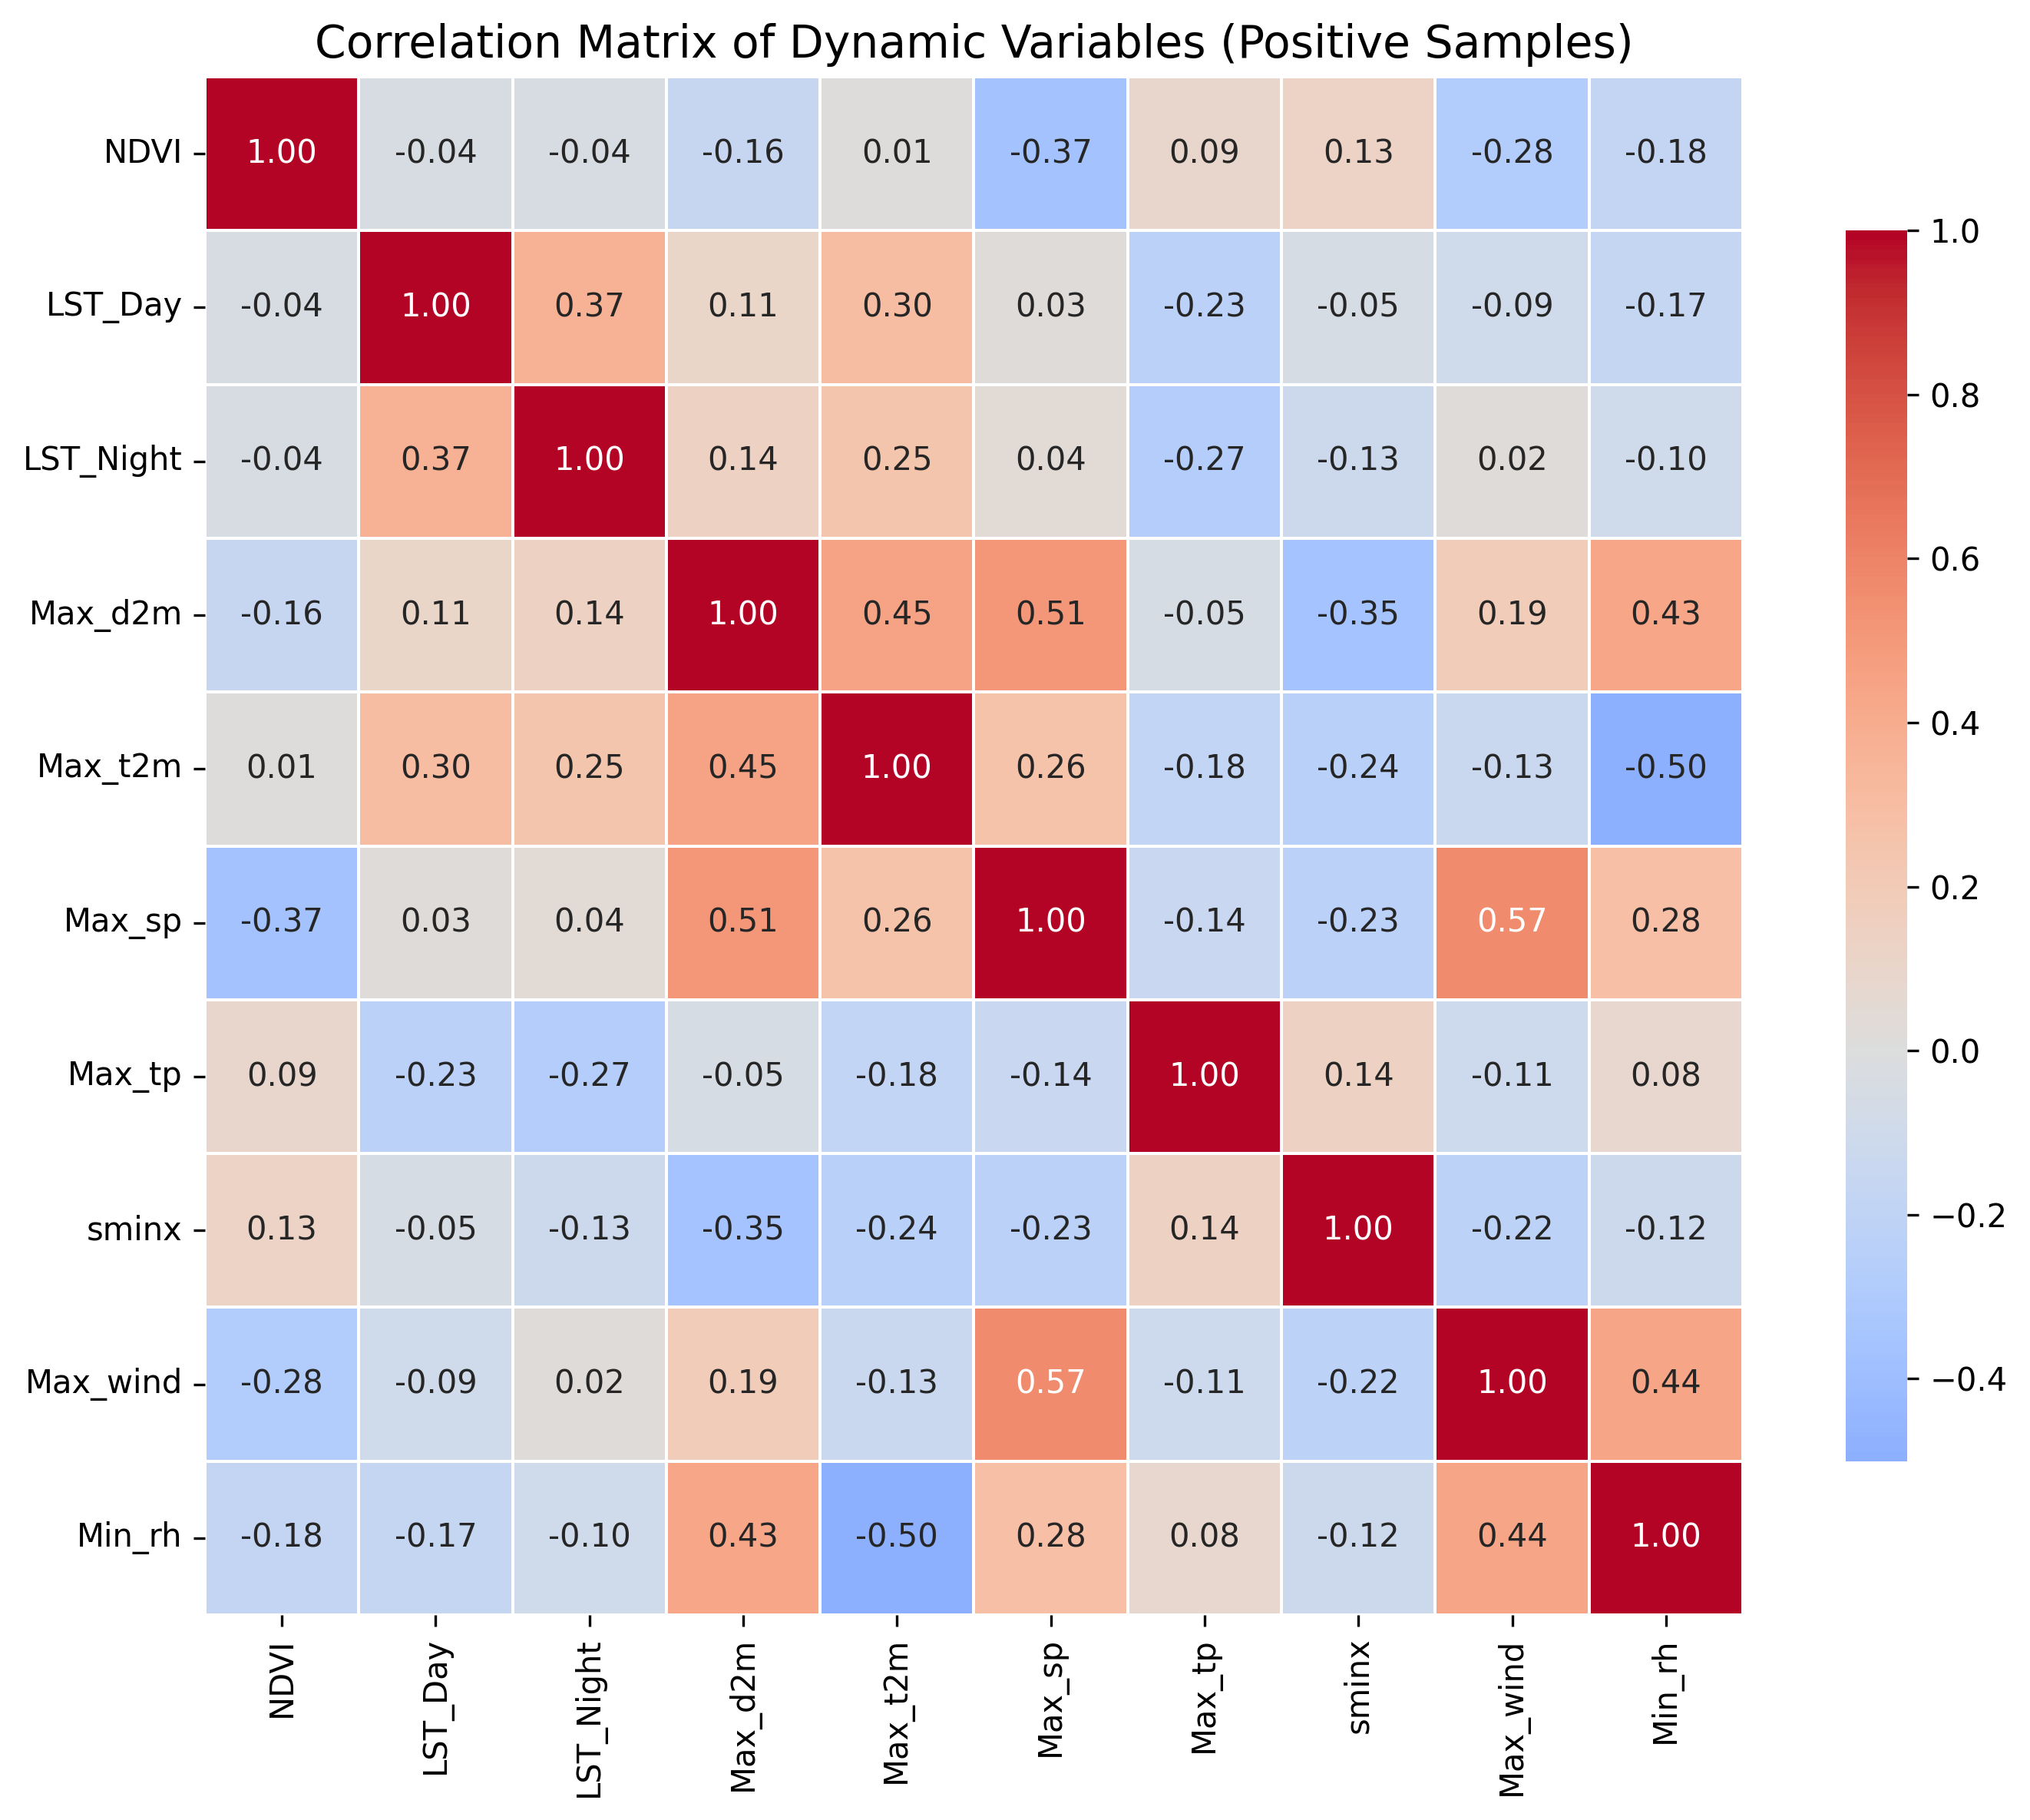
\includegraphics[width=\textwidth]{img/chap2/2-3-correlation-matrix.png}
        \caption{FireCube数据集中动态变量的皮尔逊相关性矩阵}
        \label{fig:2-3-correlation-matrix}
    \end{minipage}
    \hfill 
    \begin{minipage}{0.48\textwidth}
        \centering
        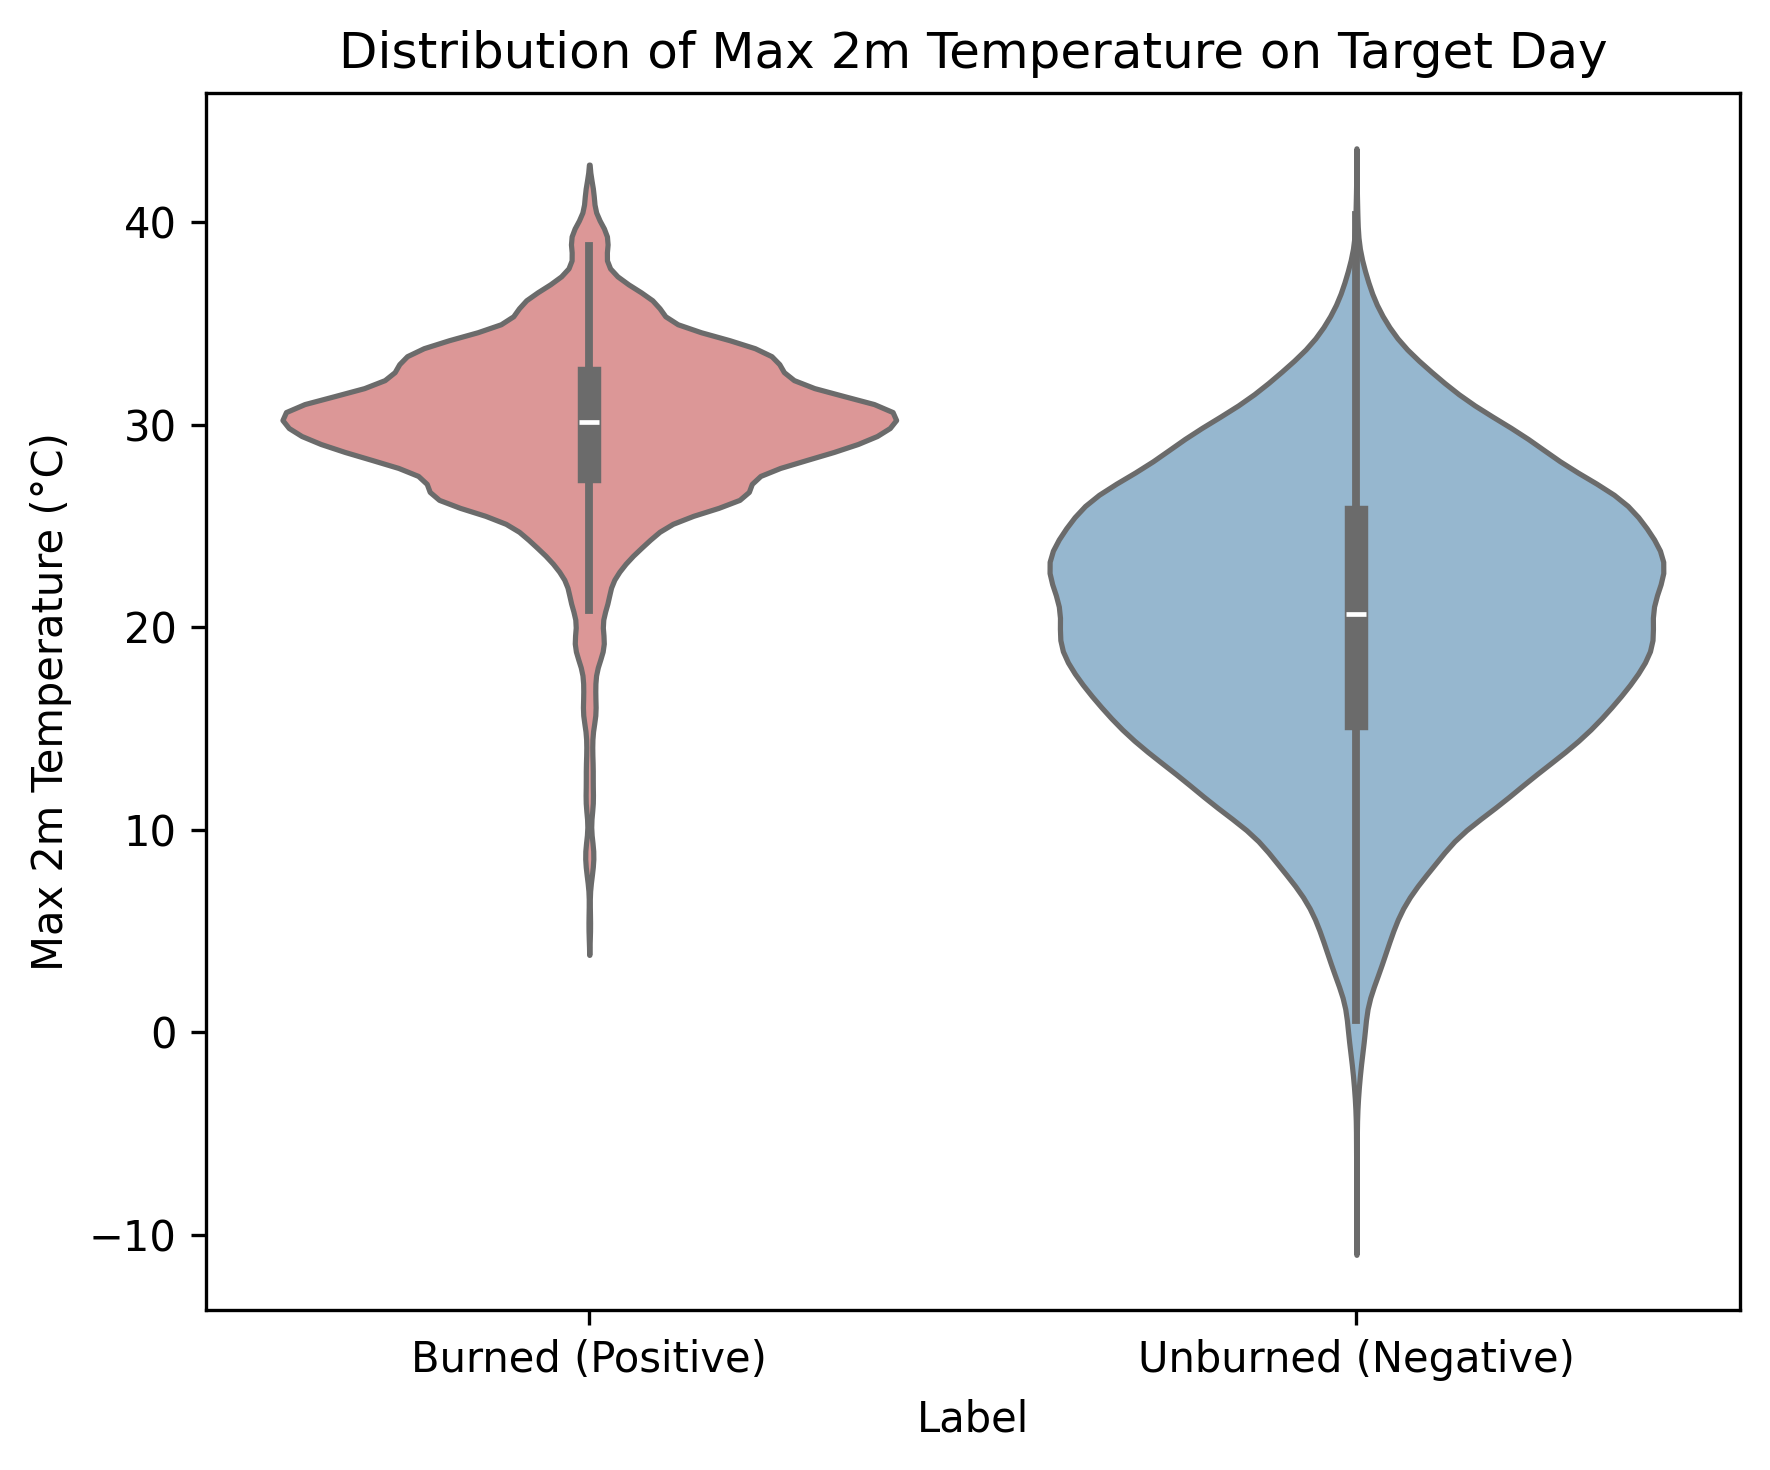
\includegraphics[width=\textwidth]{img/chap2/2-3-2m-temperature-distribution.png}
        \caption{FireCube数据集中正负样本在最高气温上的分布}
        \label{fig:2-3-2m-temperature-distribution}
    \end{minipage}
\end{figure}

图\ref{fig:2-3-2m-temperature-distribution}展示了目标日正负样本在两米处最高气温（$Max\_2m\_Temperature$）上的分布差异小提琴图。

从统计分布的形态与位置来看，起火日与非起火日的气温呈现出显著差异。未起火的负样本温度分布较为宽泛，中位数约为 21°C，反映了该地区常规气候背景下的正常自然波动。而发生野火的正样本分布较为集中，其中位数高达 30°C。这一分布特征直观地揭示了高温与野火发生的关系。同时，正负样本在$Max\_t2m$特征上的重叠度较低，表明该气象变量具有较强的判别力，验证了将其作为动态输入特征的科学性。

图\ref{fig:10-day-evolution}展示了目标日前 10 天示例气象与地表特征的时序演变图。图中实线代表所有正样本或负样本的平均值，阴影区域表示 95\% 置信区间。其中图\ref{fig:2-3-soil-moisture}展示了土壤湿度的演变轨迹，图\ref{fig:2-3-temperatures-10-days}展示了最高气温的演变轨迹。
\begin{figure}[H]
    \centering
    % 第一张子图 (a)
    \begin{subfigure}[b]{0.48\textwidth}
        \centering
        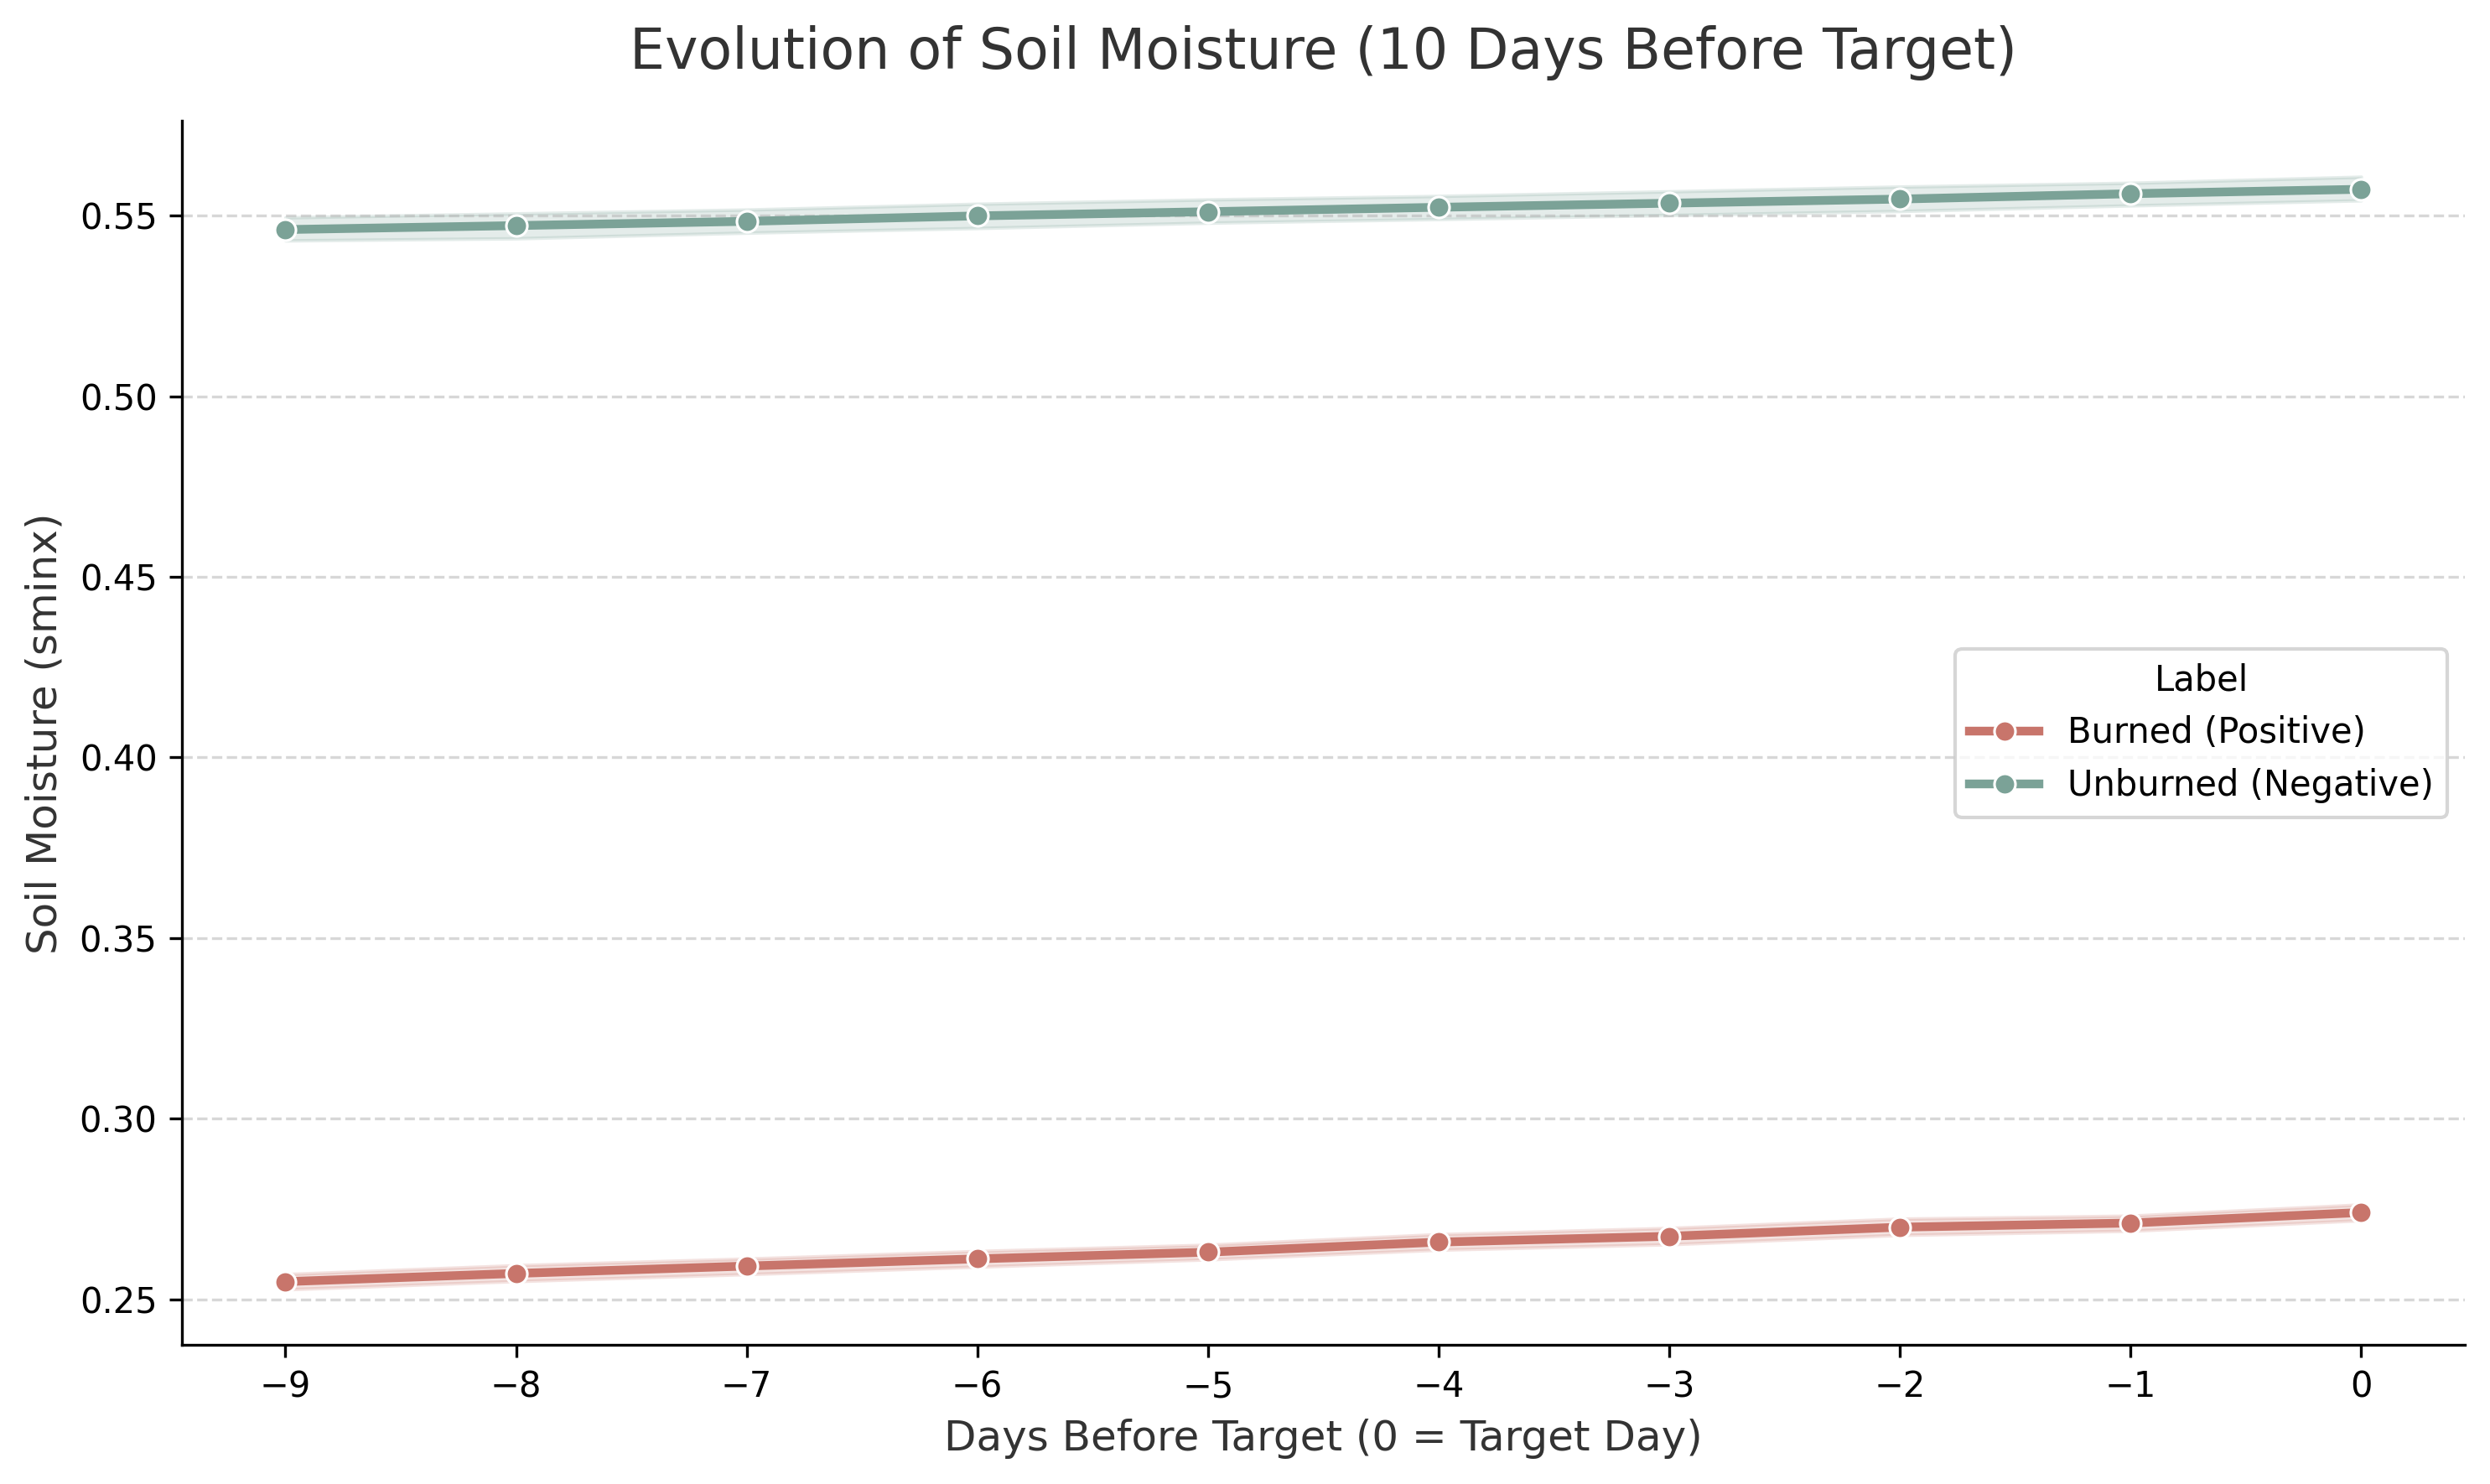
\includegraphics[width=\textwidth]{img/chap2/2-3-soil-moisture.png}
        \caption{土壤湿度的演变轨迹} % 这里写(a)图的标题，(a)会自动生成
        \label{fig:2-3-soil-moisture}
    \end{subfigure}
    \hfill 
    % 第二张子图 (b)
    \begin{subfigure}[b]{0.48\textwidth}
        \centering
        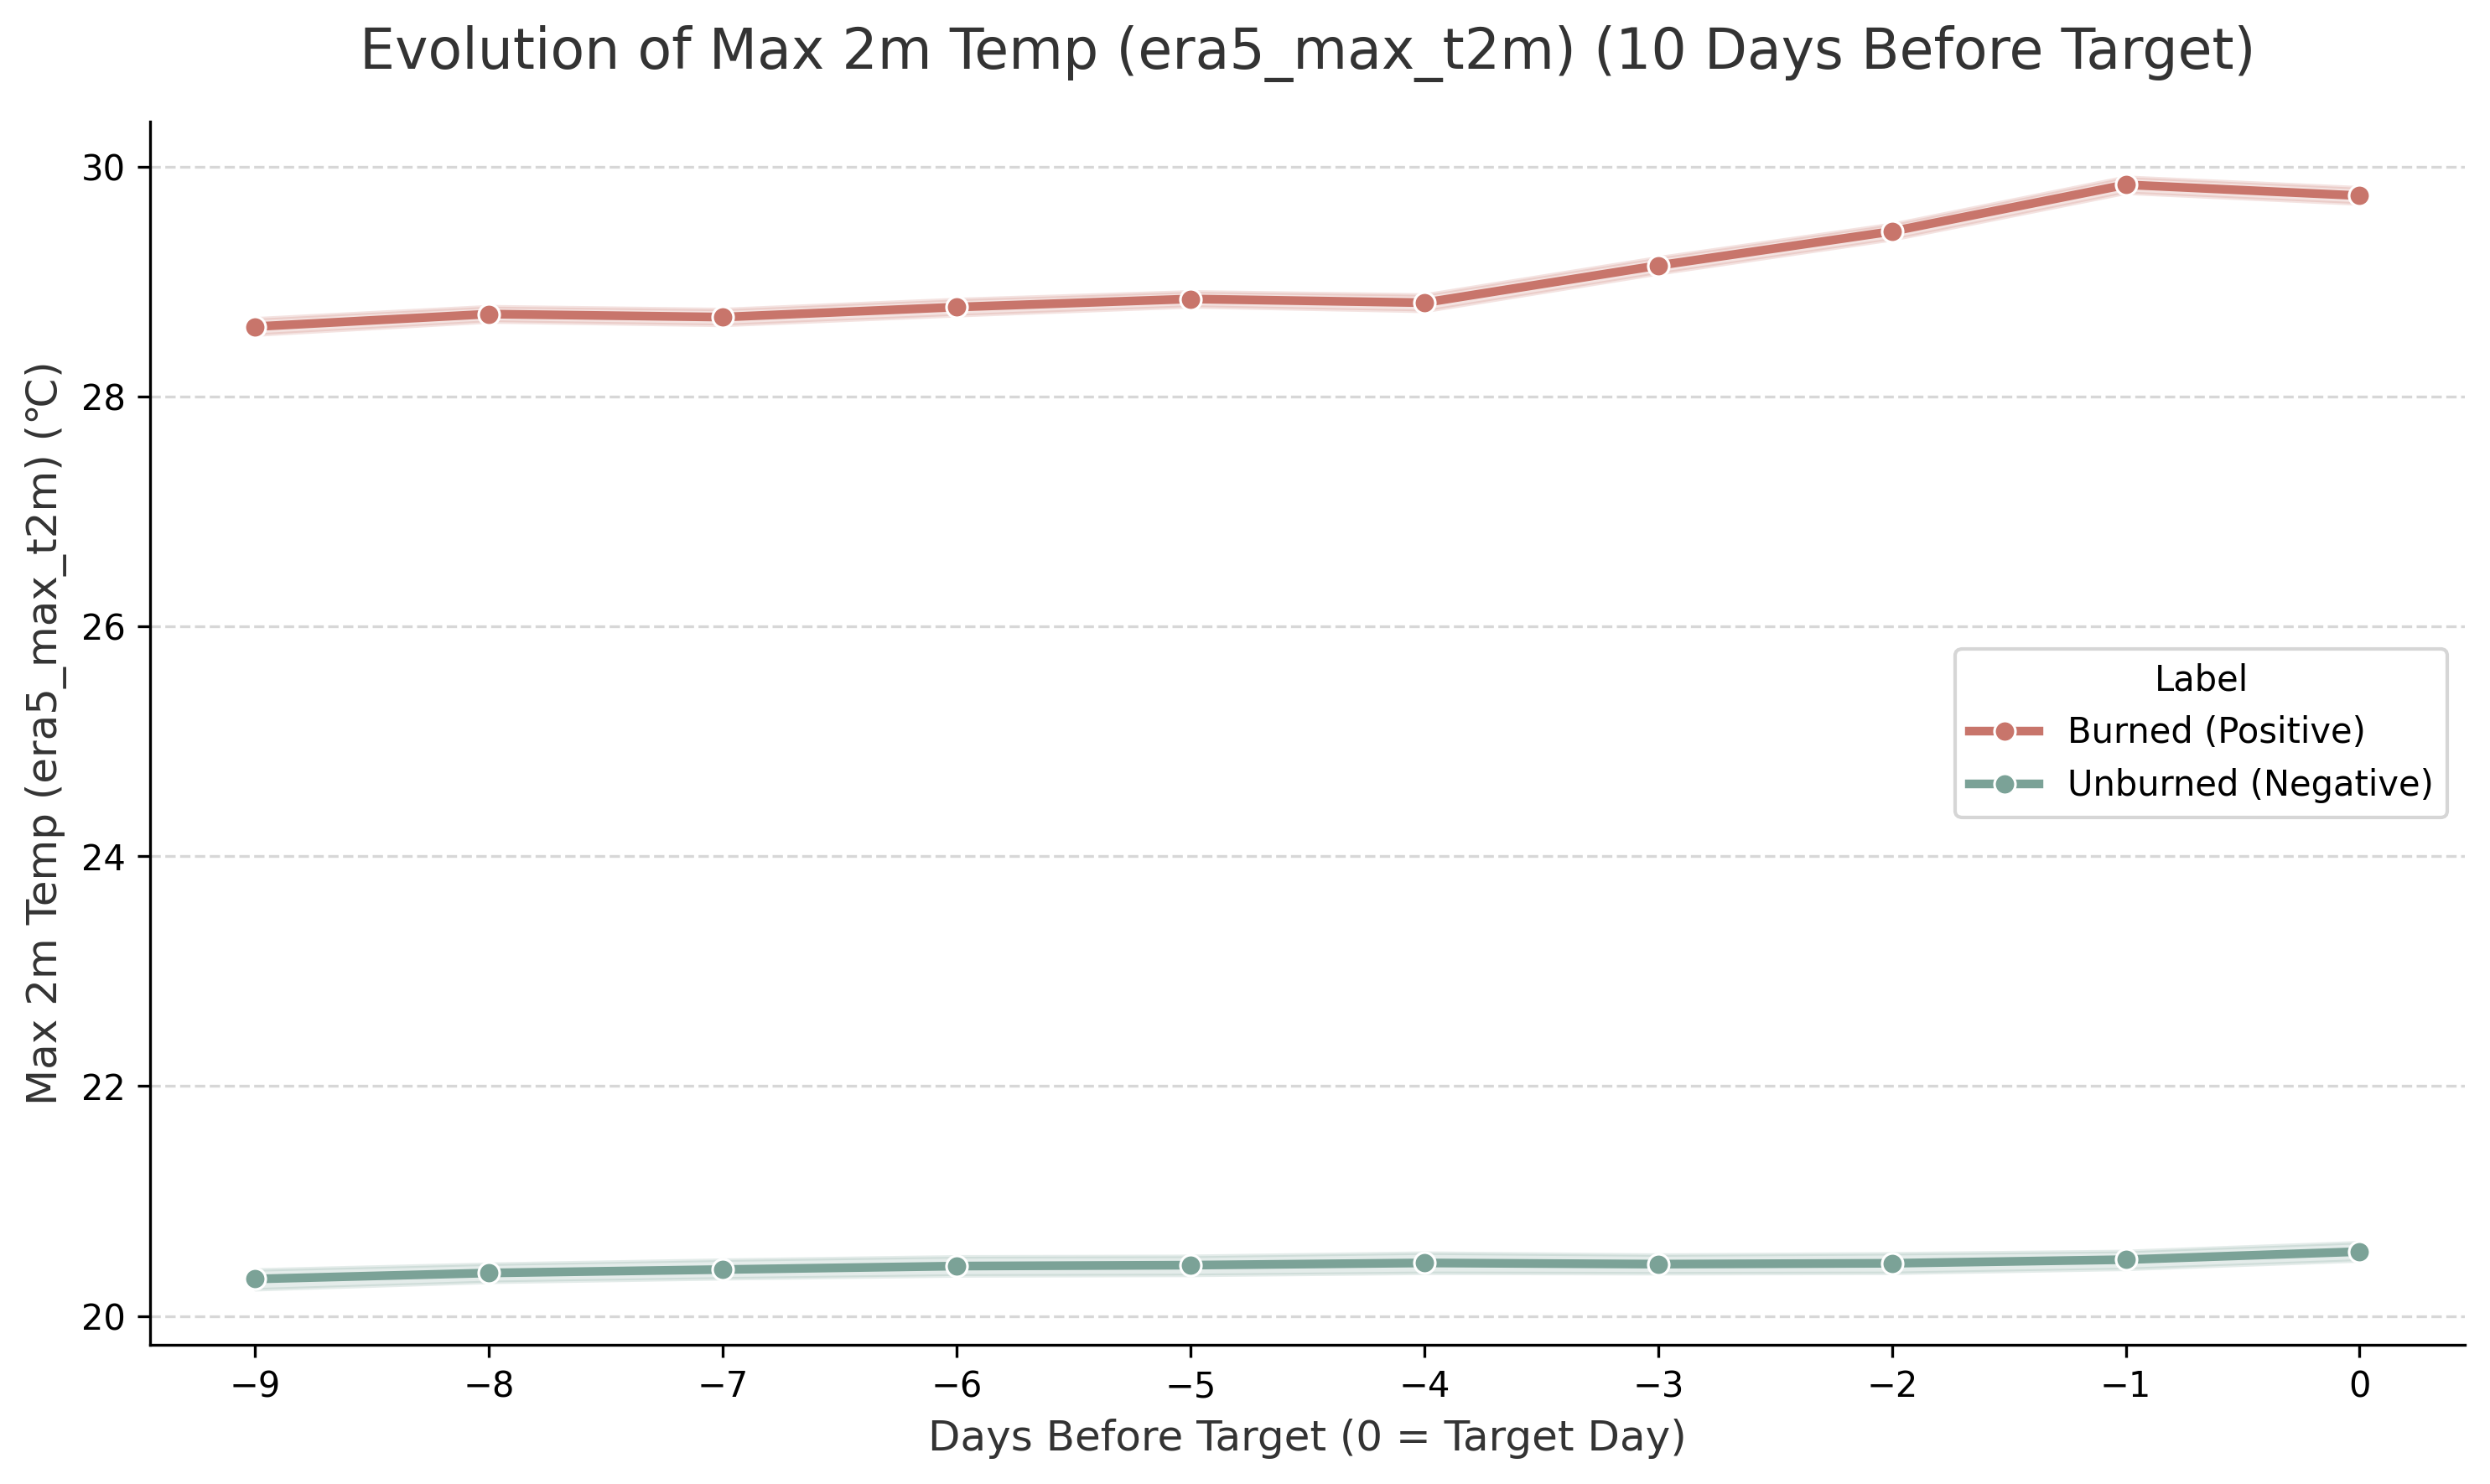
\includegraphics[width=\textwidth]{img/chap2/2-3-temperatures-10-days.png}
        \caption{最高气温的演变轨迹} % 这里写(b)图的标题，(b)会自动生成
        \label{fig:2-3-temperatures-10-days}
    \end{subfigure}
    % 整个大图的主标题
    \caption{目标日前 10 天关键气象与地表特征的时序演变图。图中实线代表正负样本的平均值，阴影区域表示 95\% 置信区间。}
    \label{fig:10-day-evolution} % 这是整个大图的引用标签
\end{figure}

在土壤湿度演变轨迹中，在绝对数值基线上，正负样本呈现出显著的差异，负样本土壤湿度大，基本在0.55左右，而正样本的土壤湿度低于0.3；在演变趋势上，负样本的土壤湿度变化范围非常小，而正样本的土壤湿度缓慢上升，变化范围相对大一些，符合野火发生的客观物理规律。在最高气温的演变轨迹中这一现象更加明显，正样本的基础最高温度比负样本高出约9°C，且负样本的温度在10天的时间尺度中几乎保持不变，而正样本呈现出温度升高的趋势。同时，土壤湿度和最高气温这两组变量之间也形成了一定的对比，在演变趋势上，表现出典型的“快慢变量耦合”特征。土壤湿度作为慢变量，在 10 天内保持相对平缓的低位震荡，表明地表已处于极度干燥的临界状态。而最高气温作为快变量，其正样本曲线在起火前的10天内呈现出一条明显的持续攀升轨迹。

上述多组特征变量分析得出的该数据集分布规律，为本研究的模型架构设计提供了直接的理论指导。具体而言，野火的发生并非由单一因素主导，本质上是静态地理约束与动态气象演变高度耦合的复杂物理过程。地表形态与植被覆盖这层静态底色，决定了灾害波及的地理空间上限，赋予了该区域特定的空间易感性；而究竟在哪个节点真正起火，则更多地取决于动态气象因子的变化。

因此，静态变量与动态变量缺一不可。这一结论直接促使本研究设计了双分支网络架构，能够同时处理不同特征，通过静态 2D 分支编码地理空间先验，利用 3D 时序分支捕获气象序列的动态演变趋势，最终在特征融合阶段实现深度融合，从而提升模型的野火预测能力。